\section{Observations}\label{sec:observations}
After implementing the different techniques for the tasks posed in section~\ref{sec:tasks}, we will now describe our observations from the analysis of these different techniques. We will elaborate on the information that was retrieved from the different techniques, list their pros and cons and come up with possible improvements for the used techniques.

\subsection{Observations Task 1}
For task 1 (as described in section~\ref{sec:task1}) we implemented a Parallel Coordinate Plot (PCP) and a Scatterplot Matrix (SM). We will first argue how both techniques performed for the subtask 1a 'analyze the relations between the different attributes'. When looking at the PCP, we first try to confirm the first question we posed int section~\ref{sec:task1}: 'is there a positive relation between the attributes \texttt{AANT\_INW} and \texttt{BEV\_DICHTH}?'. When these the axes of these two attributes are placed next to each other, it pretty quickly becomes apparent that this question can be answered positively. However, we also see that municipalities like Amsterdam and Rotterdam do not adhere to this. Apparently these municipalities cover such a large area that their vast number of inhabitants still not get them in the top of the \texttt{BEV\_DICHTH} scale. Municipalities like Leiden, 's-Gravenhage and Haarlem on the other hand have much less inhabitants, but score much higher on the \texttt{BEV\_DICHTH} scale because of their small surface area. If we then compare the attributes \texttt{OPP\_TOT} and \texttt{BEV\_DICHTH}, we can see there is a somewhat stronger (negative) relation between these two attributes.

In the SM it is much harder to see the positive relation between the attributes \texttt{AANT\_INW} and \texttt{BEV\_DICHTH}, and the negative relation between \texttt{OPP\_TOT} and \texttt{BEV\_DICHTH}. We can however quickly detect that there are some outliers in both of these relations. However, in the SM it is unfortunately not possible to retrieve which municipalities these outliers actually are by hovering over the dots. It was tried to implement this feature (similar to the tooltip hover in the PCP), but because the cursor already allows for brushing in the SM, it was not accomplished to also enable the tooltip feature. Being able to implement this tooltip feature could be regarded as a large improvement of the SM. On the other hand, when dots lie very close to each other, it may become hard to select a specific one.

When we return our attention to the PCP and want to compare other attributes with each other, we notice that quite some attributes have a few outliers that greatly enlarge the scale of the axis. These attributes include \texttt{OAD}, \texttt{AANTAL\_INW}, and \texttt{AANTAL\_HH}. Because of this, the majority of the lines cross the axis in a rather small area, making it very hard to distinguish between them. In its turn, this makes it harder to detect relations between attributes of the more 'general' municipalities. In order to solve this problem, a new feature is proposed. When a certain range of some attribute is selected, it may be convenient to stretch this range over the entire axis. In this way, more space is available to distribute the different lines, making it easier to distinguish between them. We should however ensure that the user is clearly notified of the fact that some data objects (municipalities) are left out in that specific view. The SM on its turn suffers from a similar usability problem. Because the plots are rather small, it is also hard to distinguish between different data objects. Here we propose to implement a zoom feature. Clicking on one of the plots would enlarge it to the size of the entire matrix, making it much more readable. However, as the implementation of both these proposed features was considered rather time-consuming, it was chosen not to do so.

Another observation that we can make when considering the PCP and SM for the task of comparing different attributes with each other, is that the SM makes it slightly easier to compare multiple attributes at once. Because all pairs of attributes are shown in one (or actually two) of the plots, we can quickly switch between comparing two attributes. When using the PCP, we need to shuffle around with the different axes and place the axes of two attributes next to each other in order to compare them.

Let us conclude the observations of subtask 1a with mentioning that performing this high-level task on the attribute set $S_{attr}$, mainly brings forward some rather obvious relations, or no clear relation at all. Examples of obvious relations are the positive one between \texttt{AANTAL\_INW} and \texttt{AANTAL\_HH}, and the negative relation between \texttt{OAD} and \texttt{STED}. A clearly unrelated pair of attributes would be \texttt{BEV\_DICHTH} and \texttt{P\_EENP\_HH}. Choosing different attributes might bring forward more interesting relations. However, with a lot of different attributes it might be hard to find those pairs that are truly valuable.



Next we continue to the second subtask: 'compare the attribute values of the different municipalities with each other'. Let us start with again shortly addressing the fact that because of the few significant outliers, the scale of some axes is stretched quite a lot, making it hard to distinguish between different data objects. This emphasizes that the solutions proposed earlier may be very valuable.

To answer to the specific question posed in section~\ref{sec:task1}, we can easily confirm from both the PCP and the SM that the four largest cities in the Netherlands score significantly highest on the \texttt{AANT\_INW} scale. Regarding the general, explorative question concerning interesting attribute distributions, we turn our attention to the \texttt{P\_EENP\_HH} attribute (i.e., municipalities with the highest percentage of single households). Looking at the top 8 ($>$ 50\%), we see that these spots are taken by the municipalities Wageningen, Groningen, Amsterdam, Delft, Utrecht, Nijmegen, Leiden, and Maastricht in descending order. Shortly considering this list, we may find it quite logical, as this list represents the top student cities in The Netherlands!

When comparing the values of a cluster of objects, there is one observation that can me made from both techniques. This observation can be made when comparing the cluster of the municipalities with a \texttt{STED} value of 1, with those with a \texttt{STED} value of 5. As becomes apparent from Figure~\ref{fig:sted}), the municipalities with a low \texttt{STED} value (i.e. the more urban municipalities), have much more fluctuating values for the other attributes. Municipalities with a \texttt{STED} value of 5 have values for the other attributes that lie much closer to each other. This again shows that there is a handful of municipalities that significantly influence the scaling.

\begin{figure}[h!]
    \centering
    \captionsetup{justification=centering,margin=0.5cm}
    \begin{subfigure}[t]{0.48\textwidth}
        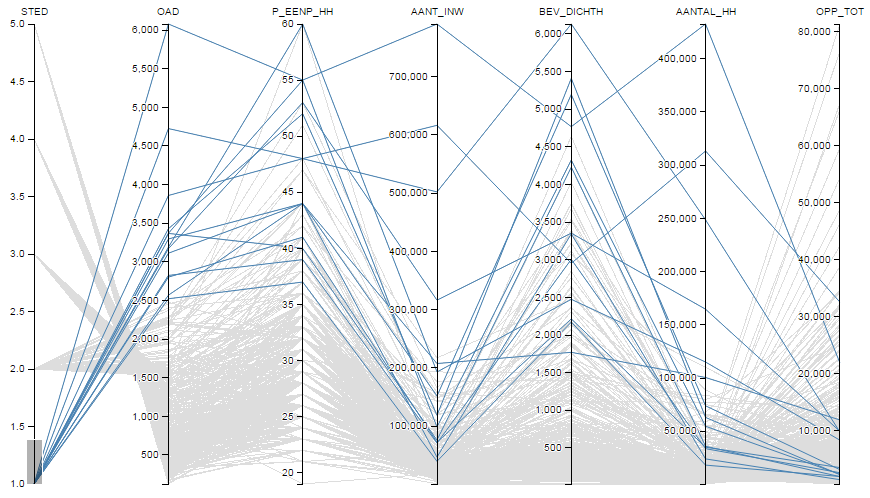
\includegraphics[width=\textwidth]{img/pcp_STED1.png}
        \caption{ }
    \end{subfigure}
    \begin{subfigure}[t]{0.48\textwidth}
        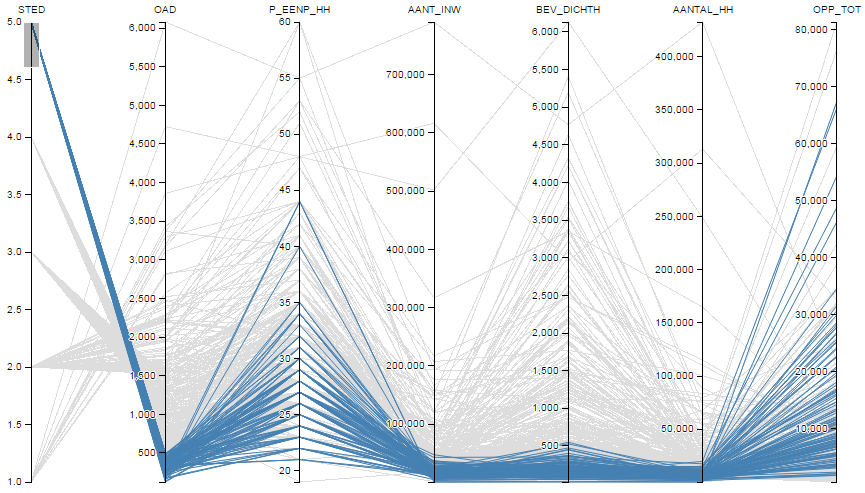
\includegraphics[width=\textwidth]{img/pcp_STED5.png}
        \caption{ }
    \end{subfigure}
    \begin{subfigure}[t]{0.48\textwidth}
        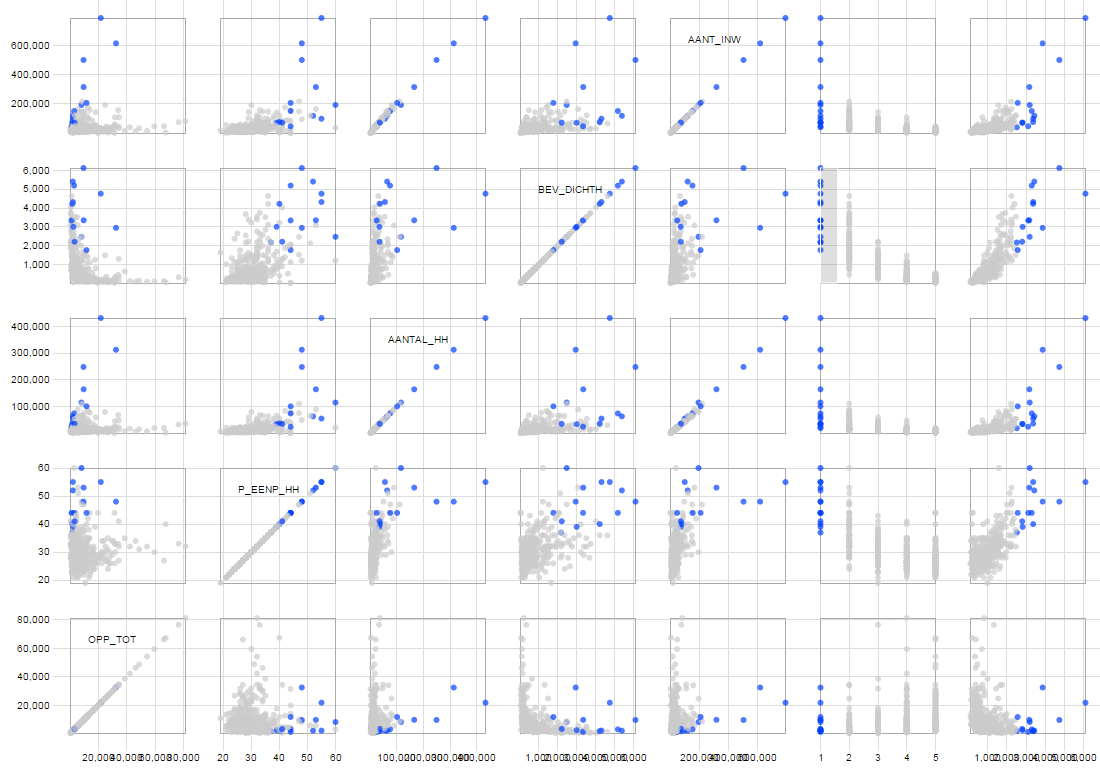
\includegraphics[width=\textwidth]{img/sm_STED1.png}
        \caption{ }
    \end{subfigure}
    \begin{subfigure}[t]{0.48\textwidth}
        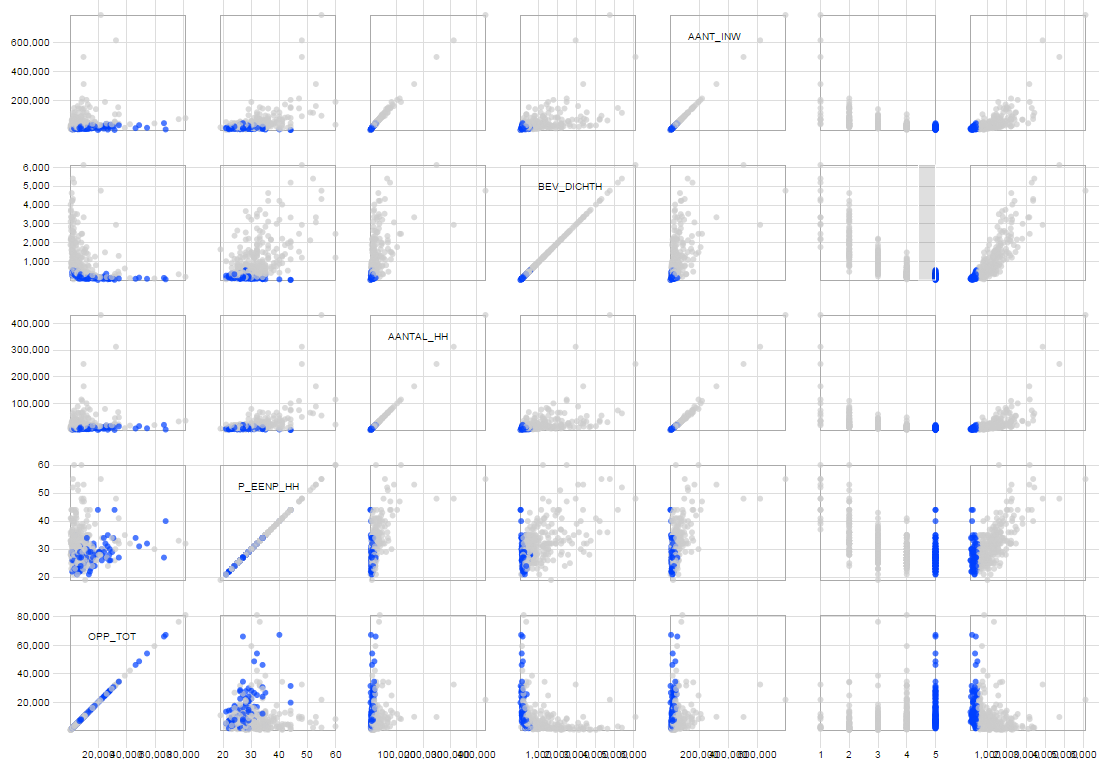
\includegraphics[width=\textwidth]{img/sm_STED5.png}
        \caption{ }
    \end{subfigure}
    \caption{Parallel Coordinate Plots highlighting the municipalities with a \texttt{STED} value of 1 (a), and a \texttt{STED} value of 5 (b), as well as the Scatterplot Matrix highlighting the municipalities with a \texttt{STED} value of 1 (c), and a \texttt{STED} value of 5 (d)}
    \label{fig:sted}
\end{figure}

Summarizing, we may conclude that both techniques are rather effective in answering the two subtasks. If we were to chose one of them, there may be  slight preference for the PCP. However, when all the proposed improvements were to be implemented, the SM might perform just as well, if not better. In general, we can conclude that this broad and high-level exploratory task may remain rather difficult with any visualization technique.


\subsection{Observations Task 2}
\todo{what information could be retrieved from the implemented technique?}
\todo{was the task accomplished?}
\todo{pros, cons, improvements}
Map vis:
schaal zou handig zijn, zien wat de min en max waarde is

welke kleuren?
wit - rood
groen - rood
